\documentclass[twocolumn,iicol,pdflatex,sn-mathphys-num]{sn-jnl}% Math and Physical Sciences Numbered Reference Style (Springer double-column design)

%%%% Standard Packages
\usepackage{graphicx}
\usepackage{multirow}
\usepackage{amsmath,amssymb,amsfonts}
\usepackage{booktabs}
\usepackage{xcolor}
%%<additional latex packages if required can be included here>
\usepackage{subcaption} 
\usepackage{tikz}
\usepackage{tikz-3dplot}
\usetikzlibrary{positioning, shapes.geometric, decorations.pathreplacing, calc}
\usepackage{bm}

% ======================================================================
% Journal-compliant large-format layout (Springer large-size design):
% text area 174 mm x 234 mm, columns 84 mm (columnsep 6 mm), so that
% single-column figures are 84 mm wide, full-width figures 174 mm wide,
% and figures are at most 234 mm high.
% ======================================================================
\geometry{%
    paperwidth=210mm,
    paperheight=297mm,
    top=26mm,
    headheight=12pt,
    headsep=5.15mm,
    text={173.35mm,233.12mm},
    marginparsep=5mm,
    marginparwidth=12mm,
    bindingoffset=6mm,
    footskip=10mm,
    columnsep=6mm,
    reversemp,
    twocolumn%
}

\begin{document}

% ======================================================================
% Frontmatter
% ======================================================================

% \title[Acoustic-Based Failure Analysis]{Acoustic-Based Failure Analysis of Power Transformers Using Multi-Modal Feature Fusion and Physics-Informed Representation Learning}

% \title[PCNN-Enhanced Multi-Modal Acoustic Fault Diagnosis]{PCNN-Enhanced Multi-Representation Fusion with Physics-Informed Learning for Power Transformer Fault Diagnosis}


% \title{Acoustic-Based Fault Diagnosis of Power Transformers Using Multi-Modal Representation Fusion Enhanced by a Pulse-Coupled Neural Network and Physics-Informed Learning}


\title{Acoustic Condition Monitoring and Fault Diagnosis of Power Transformers via Multi-Modal Fusion and Physics-Informed Representation Learning}

%% Authors -------------------------------------------------------------
\author[1]{\fnm{Chen} \sur{Yang}}\email{220242215063@ncepu.edu.cn}
\author*[1,2,3]{\fnm{Zonglong} \sur{Bai}}\email{zlbai@ncepu.edu.cn}
\author[1]{\fnm{Zhiyuan} \sur{Xie}}
\author[1]{\fnm{Chenggang} \sur{Liu}}
\author[1]{\fnm{Junyan} \sur{Zhang}}
\affil[1]{\orgdiv{Department of Electrical Engineering}, \orgname{North China Electric Power University}, \orgaddress{\city{Baoding}, \postcode{071003}, \country{China}}}

\affil[2]{\orgname{Yanzhao Electric Power Laboratory}, \orgaddress{\street{Lixing Street 666}, \city{Baoding}, \postcode{071000}, \state{Hebei}, \country{China}}}

\affil[3]{\orgname{Hebei Key Laboratory of Power Internet of Things Technology}, \orgaddress{\street{Yonghuabei Street 619}, \city{Baoding}, \postcode{071003}, \state{Hebei}, \country{China}}}


% ======================================================================
% Abstract & Keywords
% ======================================================================


\abstract{Acoustic-based power transformer fault diagnosis faces three challenges: single-modality representations, substation background noise, and scarce labeled data. This paper proposes a framework fusing Mel spectrograms with Gramian Angular Difference Fields (GADF) into three-channel images, enhanced by a pulse-coupled neural network (PCNN) for denoising and constrained by Laplacian regularization derived from the acoustic Helmholtz equation. On a real-world 220~kV transformer dataset with session-aware partitioning, the method achieves $97.26 \pm 0.82\%$ accuracy, outperforming seven representative baselines including Vision Transformer and Swin Transformer.}

\keywords{Transformer fault diagnosis, Mel spectrogram, Gramian angular difference field (GADF), pulse-coupled neural network, physics-informed representation learning, acoustic signal processing}

\maketitle

% ======================================================================
% Main Text
% ======================================================================


\section{Introduction}
Power transformers are critical assets in power systems, and continuous monitoring of their condition is essential for grid reliability \cite{HE2026119781,Zhao2026}. Acoustic-based diagnosis is attractive owing to non-contact measurement, ease of deployment, and low cost, yet three challenges remain: single-modality time--frequency representations capture only partial fault signatures; substation background noise degrades classification reliability; and scarce labeled fault data limit the generalization of purely data-driven models.

Time--frequency methods such as the Mel spectrogram \cite{10606641}, wavelet denoising \cite{4265659}, STFT analysis \cite{7558591}, and Gramian angular field (GAF) encoding \cite{9760386} provide informative input representations, while CNNs \cite{11014495}, Vision Transformers (ViT) \cite{dosovitskiy2021vit}, EfficientNet \cite{tan2019efficientnet}, and Swin Transformer \cite{liu2021swin} have advanced classification performance. However, conventional pipelines remain purely data-driven and overfit on small, noisy datasets. Physics-informed neural networks (PINNs) integrate domain knowledge into training \cite{9903391,r4} and have been applied to dissolved gas analysis \cite{10964340} and wind turbine monitoring \cite{11027711}. In acoustic diagnosis, the pressure field in the transformer tank obeys the wave equation, which in the source-free low-frequency limit reduces to the Laplace equation $\nabla^2 p \approx 0$: fault-free acoustic fields are spatially smooth, so penalizing the Laplacian of the learned features provides a physically grounded prior.

This paper proposes a framework integrating multi-modal fusion, biologically inspired denoising, and physics-informed representation learning. The main contributions are:

\begin{enumerate}
	\item \textbf{Multi-modal fusion and PCNN enhancement:} Mel spectrograms, GADF, and their pixel-wise difference are fused into a three-channel representation; gamma correction ($\gamma = 1.7$) and a pulse-coupled neural network (PCNN) enhance low-energy regions and suppress background noise.
	
	\item \textbf{Physics-informed representation learning:} Laplacian smoothness regularization, derived from the Helmholtz equation under the source-free approximation, is enforced directly in the feature space of a CNN, avoiding collocation-point PDE solving.
	
	\item \textbf{Rigorous validation:} Component-wise ablation, five-fold cross-validation with session-aware splits, and comparison with seven representative methods demonstrate state-of-the-art performance.
\end{enumerate}

The remainder of this paper is organized as follows: Section~\ref{section2} introduces the time--frequency representations, Section~\ref{section3} the fusion and PCNN enhancement, Section~\ref{section4} the physics-informed framework, Section~\ref{section5} the experiments, and Section~\ref{section6} concludes. The overall framework is illustrated in Fig.~\ref{fig0}.

\begin{figure*}[t]
	\centering
	\includegraphics[width=1.0\linewidth]{pinn-alexnet}
	\caption{Overall framework of the proposed transformer fault diagnosis method. The pipeline consists of four stages: (1) multi-modal time--frequency representation via Mel spectrogram and GADF, (2) three-channel feature fusion with gamma correction, (3) PCNN-based feature enhancement, and (4) physics-informed AlexNet-SE classification with Laplacian regularization.}
	\label{fig0}
\end{figure*}

\section{Time-Frequency Domain Representation}
\label{section2}

\subsection{Mel Spectrogram}
\label{subsec1}
The Mel spectrogram emulates the non-linear frequency perception of the human auditory system \cite{10768989}. The mapping from linear frequency $f$ to the Mel scale is \cite{11097896}
\begin{equation}
	f_{\text{mel}} = 2595 \log_{10}\!\left(1 + \frac{f}{700}\right)
\end{equation}
As the physical frequency increases, the Mel scale grows sub-linearly, yielding higher resolution in the low-frequency bands where transformer acoustic fault signatures concentrate, which motivates the Mel spectrogram as the primary spectral representation.

For each 1-second segment, the short-time Fourier transform (STFT) is computed with a 25~ms Hamming window and 50\% overlap, then passed through a Mel filter bank of 128 triangular filters spaced uniformly on the Mel scale; the response $H_m(k)$ of the $m$-th filter rises linearly from the lower corner frequency $f(m-1)$ to the center $f(m)$ and falls to the upper corner $f(m+1)$ \cite{r1}. The resulting Mel spectrogram of a normal transformer is illustrated in Fig.~\ref{fig1}.

\begin{figure*}[htbp]
	\centering
	\begin{subfigure}[b]{0.42\textwidth}
		\centering
		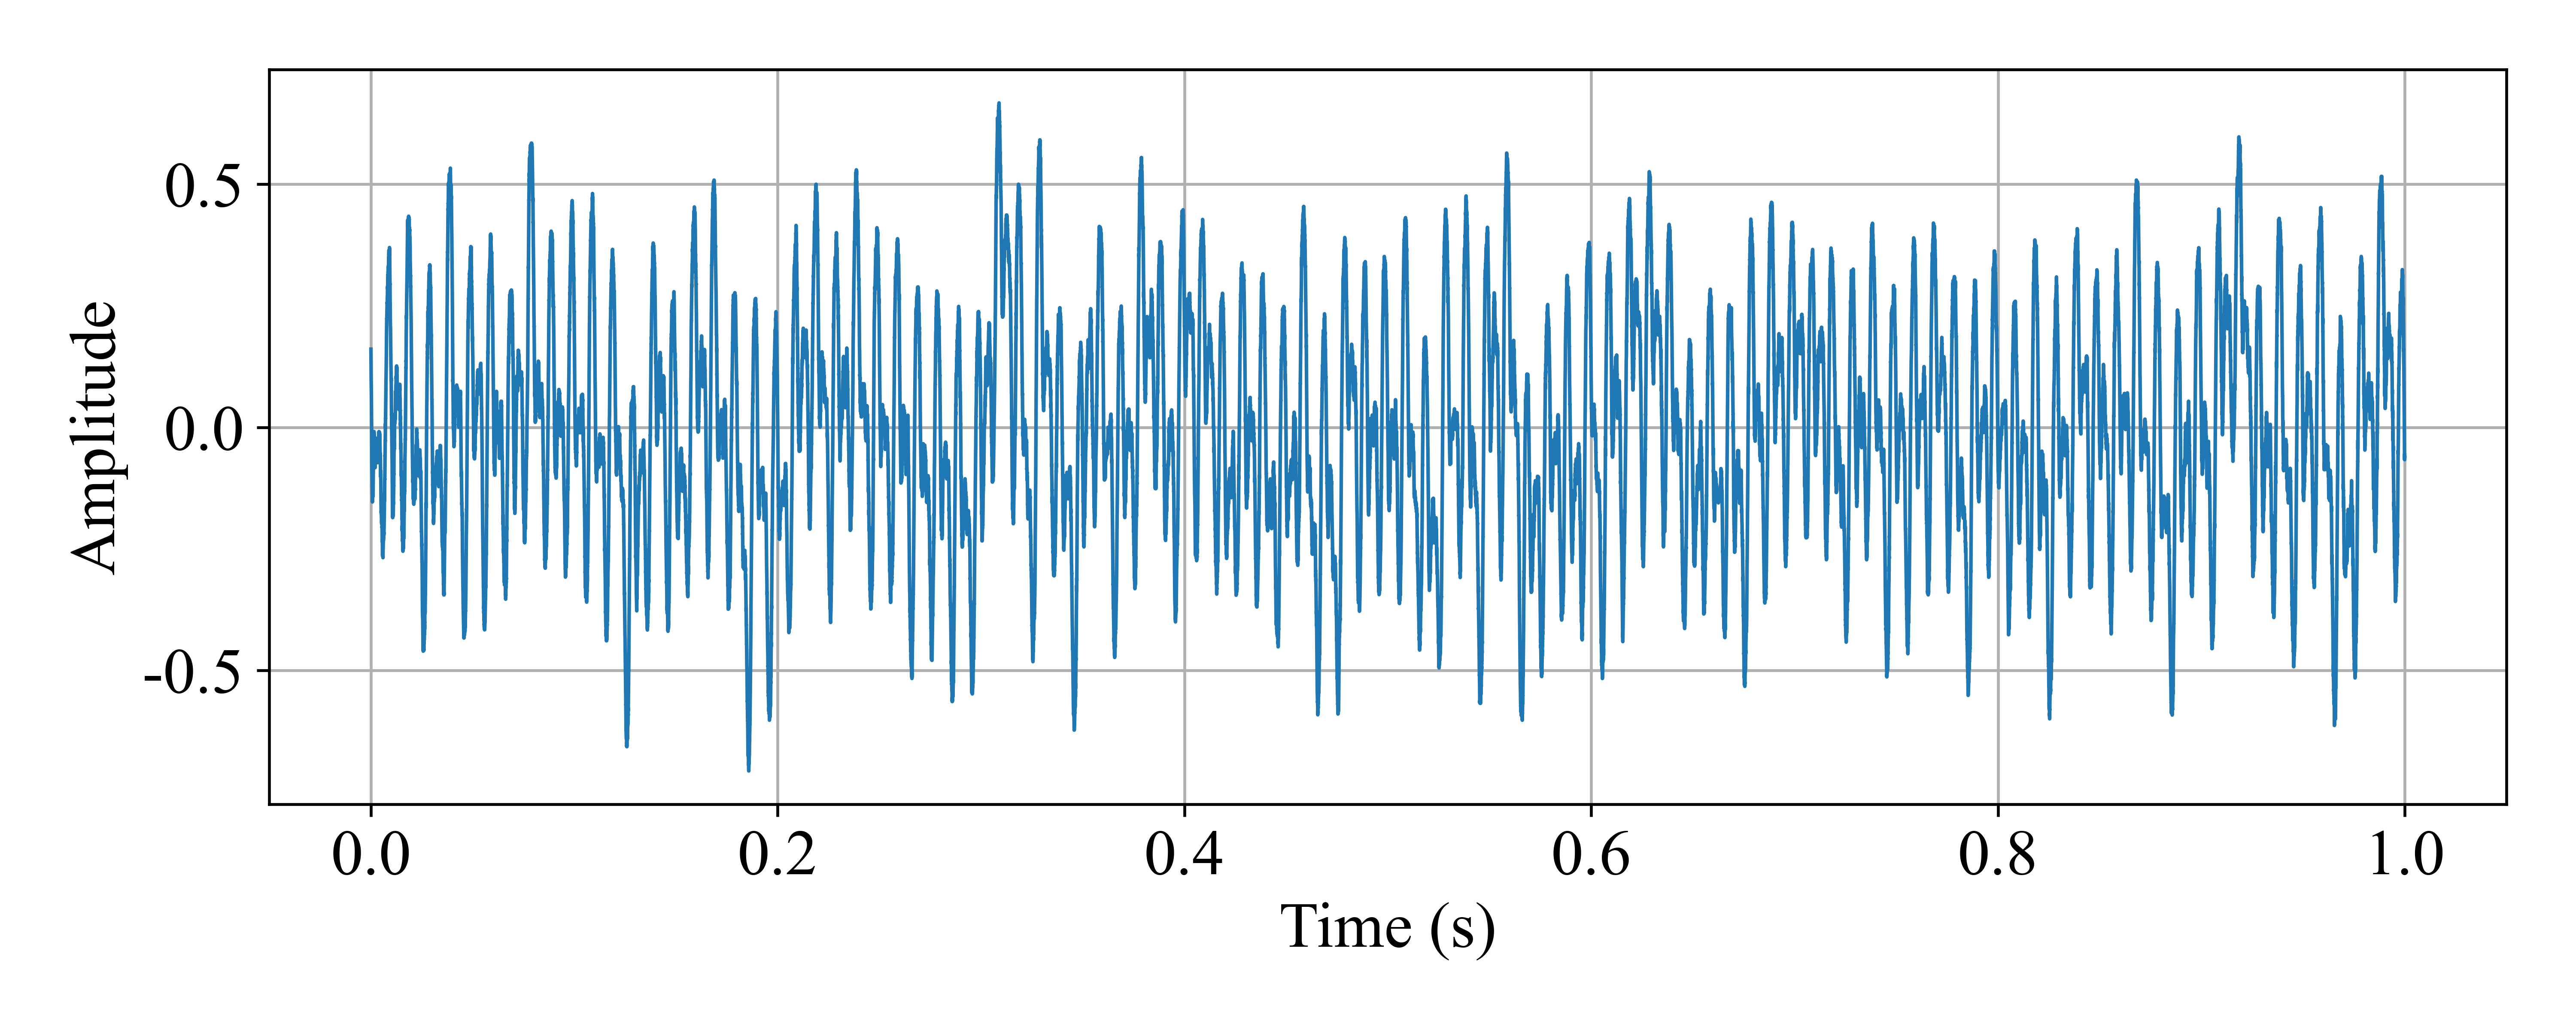
\includegraphics[width=\textwidth]{Normal.png}
		\caption*{(a)} 
	\end{subfigure}
	\hfill
	\begin{subfigure}[b]{0.42\textwidth}
		\centering
		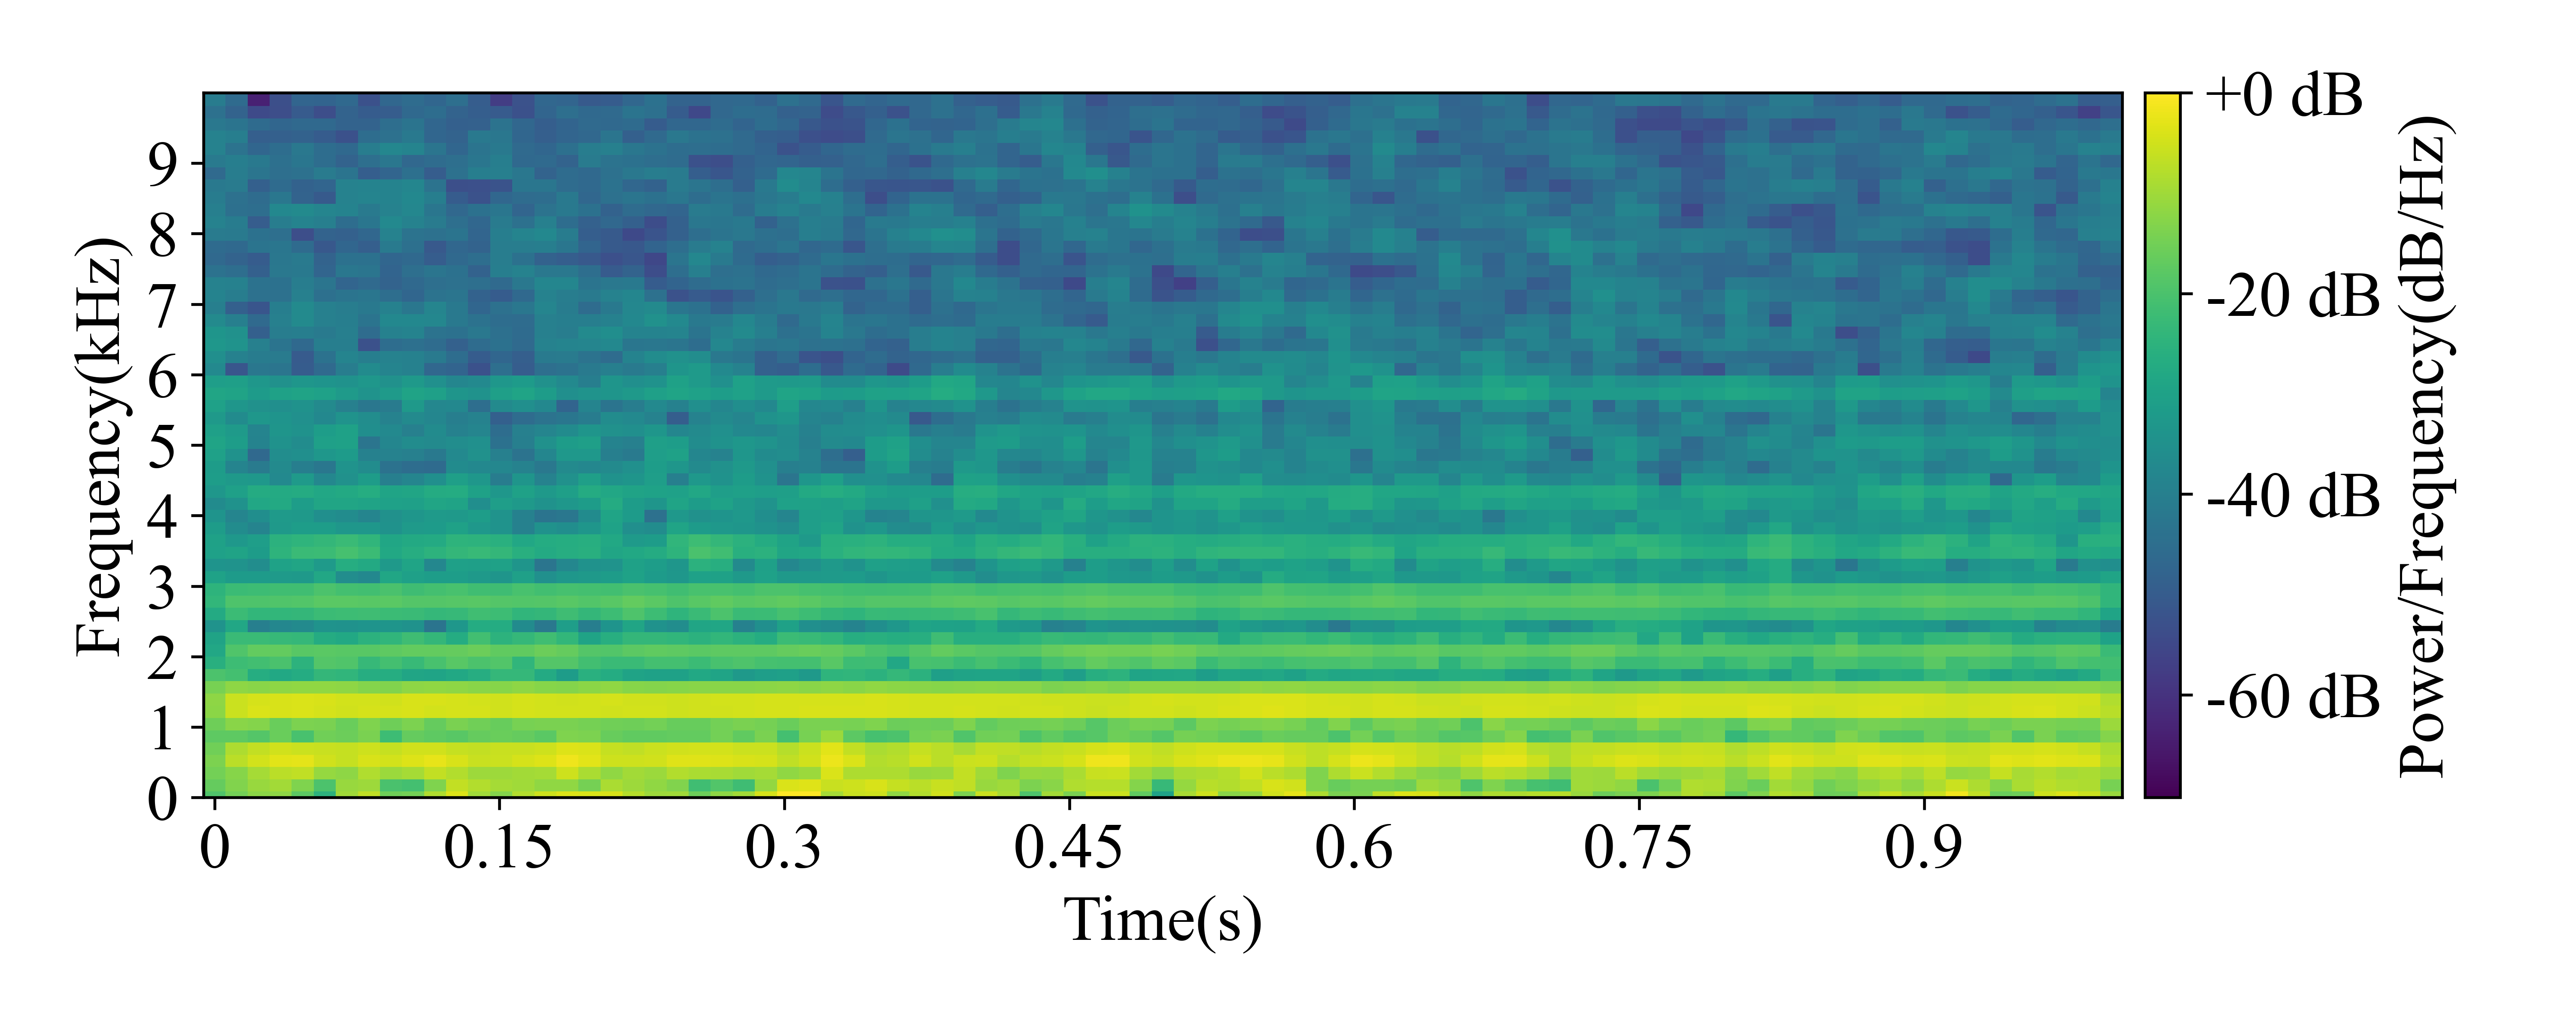
\includegraphics[width=\textwidth]{Mel_spectrogram.png}
		\caption*{(b)}
	\end{subfigure}
	\caption{Transformer acoustic signal under normal operating conditions. (a) Time-domain waveform. (b) Corresponding Mel spectrogram.}
	\label{fig1}
\end{figure*}

\subsection{Gramian Angular Field}
The Gramian Angular Field (GAF) is a method for encoding one-dimensional time series into two-dimensional image representations that preserve the temporal correlation structure \cite{10114345}. By representing time-series values in polar coordinates and computing pairwise trigonometric interactions, GAF produces images where each element $(i,j)$ encodes the temporal relationship between time steps $i$ and $j$. Two variants exist, i.e., the Gramian Angular Summation Field (GASF) based on $\cos(\phi_i + \phi_j)$, and the Gramian Angular Difference Field (GADF) based on $\sin(\phi_i - \phi_j)$ \cite{10281942}. The encoding procedure involves three steps:

\begin{enumerate}
	\item \textbf{Normalization:} A univariate time series $X = \{x_1, \ldots, x_n\}$ is rescaled to $[-1, 1]$ via min--max normalization,
	\begin{equation}
		\resizebox{0.8\columnwidth}{!}{$\tilde{x}_i = \dfrac{(x_i - \min X) + (x_i - \max X)}{\max X - \min X}, \quad i = 1, 2, \ldots, n$}
	\end{equation}
	
	\item \textbf{Polar encoding:} Each normalized value is mapped to polar coordinates, with $\phi_i = \arccos(\tilde{x}_i) \in [0, \pi]$ encoding the amplitude and $r_i = i/n$ encoding the temporal position, so temporal ordering is preserved.
	
	\item \textbf{Gramian matrix construction:} The GASF $\bm{G}_s$ and GADF $\bm{G}_d$ are $n \times n$ matrices with entries
	\begin{equation}
		\begin{aligned}
			[\bm{G}_s]_{i,j} &= \cos(\phi_i + \phi_j), \\
			[\bm{G}_d]_{i,j} &= \sin(\phi_i - \phi_j),
		\end{aligned}
	\end{equation}
	for $i, j = 1, \ldots, n$.
\end{enumerate}

GADF is more sensitive to local phase variations than GASF \cite{8975572}; both variants are compared experimentally in Section~\ref{exp1}, and Fig.~\ref{fig2} shows them for a normal-condition signal.

\begin{figure*}[t]
	\centering
	\subfloat[]{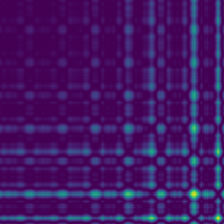
\includegraphics[width=0.42\textwidth]{GASF}}\hfill
	\subfloat[]{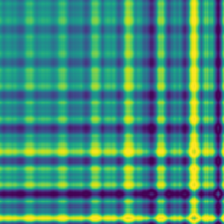
\includegraphics[width=0.42\textwidth]{GADF}}
	\caption{GAF representations of a transformer acoustic signal: (a) GASF, (b) GADF. The GADF representation exhibits stronger contrast in the off-diagonal texture patterns, which capture transient fault signatures more distinctly.}
	\label{fig2}
\end{figure*}


\section{Multi-Modal Feature Extraction and Fusion}
\label{section3}
\subsection{Mel-GAF Three-Channel Fusion Strategy}
Feature fusion combines complementary information from heterogeneous representations to improve performance \cite{10902169}. For each 1-second segment, the Mel spectrogram $\bm{M} \in \mathbb{R}^{H \times W}$ and the GADF matrix $\bm{G}_d \in \mathbb{R}^{n \times n}$ are resized to $224 \times 224$ pixels with bicubic interpolation, normalized to $[0, 1]$, and fused into a three-channel image

\begin{equation}
	\resizebox{0.8\columnwidth}{!}{$\bm{I}_{\text{fused}} = \begin{bmatrix}
		\bm{I}_R \\ \bm{I}_G \\ \bm{I}_B
	\end{bmatrix} = \begin{bmatrix}
		\bm{M}_{\text{norm}} \\
		\bm{G}_{d,\text{norm}} \\
		|\bm{M}_{\text{norm}} - \bm{G}_{d,\text{norm}}|
	\end{bmatrix},$}
\end{equation}
where the R channel is the Mel spectrogram, the G channel is the GADF texture, and the B channel is their pixel-wise absolute difference. The difference channel highlights regions where spectral energy and temporal correlation diverge---i.e., anomalous fault signatures---and provides an explicit cross-modal complementarity signal for the CNN \cite{9673131}.

\subsection{Image Preprocessing and Gamma Correction}
In the raw fused images, the Mel channel suffers from a large dynamic range: low-energy bands are orders of magnitude weaker than dominant harmonics and appear visually indistinct. Gamma correction \cite{8362729},
\begin{equation}
	I_{\text{out}} = c \cdot I_{\text{in}}^{\gamma},
\end{equation}
with $c = 1$, expands the dynamic range of dark regions for $\gamma > 1$, enhancing low-energy contrast. Grid search over $\gamma \in [0.5, 3.0]$ selected $\gamma = 1.7$: lower values provided insufficient enhancement and higher values over-saturated high-energy regions. Fig.~\ref{fig3} compares the fused image before and after correction.

\begin{figure*}[t]
	\centering
	\subfloat[]{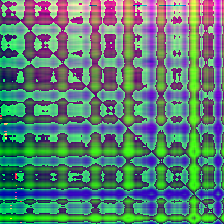
\includegraphics[width=0.42\textwidth]{1}}\hfill
	\subfloat[]{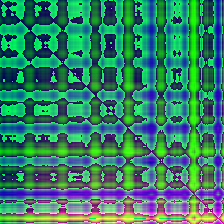
\includegraphics[width=0.42\textwidth]{2}}
	\caption{Comparison of the fused Mel-GADF image (a) before and (b) after gamma correction with $\gamma = 1.7$. The corrected image exhibits enhanced contrast in low-energy regions while preserving high-energy structural details.}
	\label{fig3}
\end{figure*}


\subsection{Multi-Condition Fused Representations}
Fig.~\ref{fig4} presents the fused representations for five transformer operating conditions: normal (N0), harmonic distortion (N1), DC-bias (N2), mechanical looseness (N3), and partial discharge (N4). Each fault type induces distinct patterns in the spectral energy distribution (R channel) and the temporal correlation structure (G channel), with their divergence captured in the B channel; the fused images are visually richer and more discriminative than single-modality representations.

\begin{figure*}[htbp]
	\centering
	\begin{tabular}{c@{\hspace{0.3cm}}ccccc}
		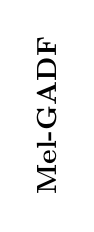
\begin{tikzpicture}
			\node[align=right] {\rotatebox{90}{\textbf{Mel-GADF}}}; 
		\end{tikzpicture}
		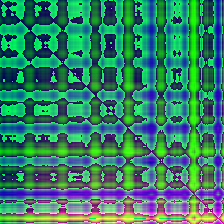
\includegraphics[width=0.15\textwidth]{Normal_part0_1} &
		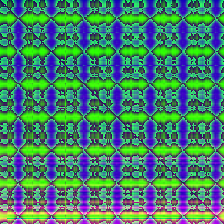
\includegraphics[width=0.15\textwidth]{G4_10pSeventhHarmonic_1_1} &
		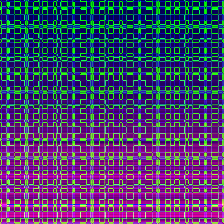
\includegraphics[width=0.15\textwidth]{DCBias2_1_1} &
		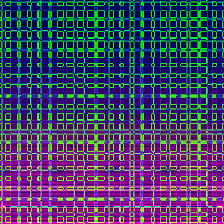
\includegraphics[width=0.15\textwidth]{Loosen1_1_1} &
		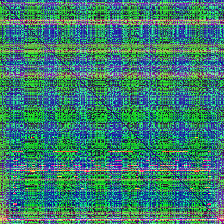
\includegraphics[width=0.15\textwidth]{PartialDischarge1_1_1} \\
	\end{tabular}
	\vspace{0.15cm}
	\begin{tikzpicture}
		\draw[dash pattern=on 8pt off 2pt, line width=0.6pt,blue] (0,0) -- (\textwidth,0);
	\end{tikzpicture}
	\vspace{0.15cm}
	\begin{tabular}{c@{\hspace{0.3cm}}ccccc}
		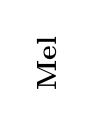
\begin{tikzpicture}
			\node[align=right] {\rotatebox{90}{\textbf{Mel}}};
		\end{tikzpicture}
		\subfloat[]{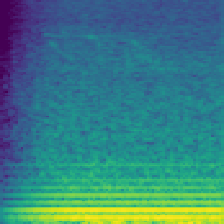
\includegraphics[width=0.15\textwidth]{Normal_Mel.png}} &
		\subfloat[]{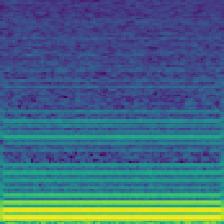
\includegraphics[width=0.15\textwidth]{Harmonic_Mel.png}} &
		\subfloat[]{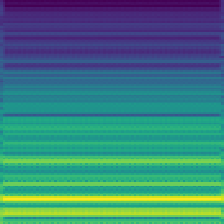
\includegraphics[width=0.15\textwidth]{DCBias_Mel.png}} &
		\subfloat[]{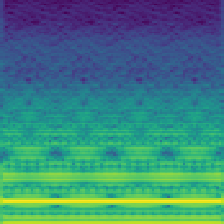
\includegraphics[width=0.15\textwidth]{Loosen_Mel.png}} &
		\subfloat[]{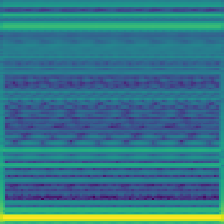
\includegraphics[width=0.15\textwidth]{PartialDischarge_Mel.png}} \\
	\end{tabular}
	\caption{Multi-modal representations across five transformer operating conditions. Top: Mel-GADF fusion (proposed); Bottom: Mel spectrogram alone. Conditions (left to right): (a) Normal, (b) Harmonic distortion, (c) DC-bias, (d) Mechanical looseness, (e) Partial discharge.}
	\label{fig4}
\end{figure*}

\subsection{PCNN-Based Feature Enhancement}
Pulse-Coupled Neural Networks (PCNNs) are biologically inspired models that emulate synchronized pulse firing in the mammalian visual cortex \cite{4305279}. Their iterative, locally coupled dynamics are effective for noise suppression and edge-preserving image enhancement \cite{10341267}. For each pixel $(i, j)$, the dynamics comprise:

\begin{enumerate}
	\item \textbf{Feeding input:}
	\begin{equation}
		F_{i,j}[n] = e^{-\alpha_{F}} F_{i,j}[n - 1] + V_{F} \, S_{i,j}
	\end{equation}
	where $S_{i,j}$ is the external stimulus (pixel intensity), $\alpha_F$ the feeding decay, $V_F$ the input gain, and $n$ the iteration step.
	
	\item \textbf{Linking modulation:}
	\begin{multline}
		L_{i,j}[n] = e^{-\alpha_L} L_{i,j}[n-1] \\
		+ V_L \sum_{(k,l) \in \mathcal{N}(i,j)} W_{i,j;k,l} \, Y_{k,l}[n-1]
	\end{multline}
	where $\mathcal{N}(i,j)$ is the local receptive field and $W_{i,j;k,l}$ a Gaussian coupling kernel weighting the binary pulses $Y_{k,l}$ of neighboring neurons.
	
	\item \textbf{Internal activity and pulse generation:}
	\begin{equation}
		U_{i,j}[n] = F_{i,j}[n] \left(1 + \beta \, L_{i,j}[n]\right)
	\end{equation}
	\begin{equation}
		Y_{i,j}[n] = 
		\begin{cases} 
			1, & \text{if } U_{i,j}[n] > T_{i,j}[n] \\
			0, & \text{otherwise}
		\end{cases}
	\end{equation}
	\begin{equation}
		T_{i,j}[n] = e^{-\alpha_T} T_{i,j}[n-1] + V_T \, Y_{i,j}[n]
	\end{equation}
	where $U_{i,j}[n]$ is the total internal excitation, $Y_{i,j}[n]$ the binary pulse output, $T_{i,j}[n]$ the dynamic threshold, and $\beta$ the linking strength.
\end{enumerate}

Synchronized firing suppresses isolated low-magnitude noise pixels while amplifying spatially coherent structures such as harmonic lines and fault-induced spectral ridges. Fig.~\ref{fig5} shows the effect of the initial threshold $V_T$: noise is progressively suppressed as $V_T$ increases, and $V_T = 0.8$ with $N = 10$ iterations are chosen by parameter analysis; at $V_T \geq 1.0$ firing is nearly fully inhibited.

\begin{figure*}[t]
	\centering
	\subfloat[]{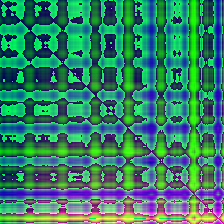
\includegraphics[width=0.20\textwidth]{VT_Normal_part0}}\hfill
	\subfloat[]{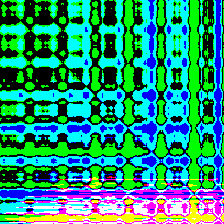
\includegraphics[width=0.20\textwidth]{Normal_part04}}\hfill
	\subfloat[]{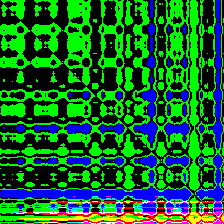
\includegraphics[width=0.20\textwidth]{Normal_part06}}\hfill
	\subfloat[]{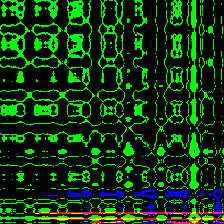
\includegraphics[width=0.20\textwidth]{Normal_part08}}
	\caption{Effect of PCNN processing with different initial thresholds $V_T$ on the Mel-GADF image: (a) Original (no PCNN), (b) $V_T = 0.4$, (c) $V_T = 0.6$, (d) $V_T = 0.8$. Higher thresholds yield stronger noise suppression while preserving edge structures.}
	\label{fig5}
\end{figure*}


\section{Physics-Informed Representation Learning for Fault Diagnosis}
\label{section4}
\subsection{Physical Motivation: Acoustic Wave Propagation in Transformer Tanks}

The physical prior underlying the proposed regularizer follows from sound propagation in the transformer tank. The acoustic pressure field $p(\mathbf{x}, t)$, generated by mechanical vibrations of the core and windings, obeys the linear wave equation:
\begin{equation}
	\frac{\partial^2 p(\mathbf{x}, t)}{\partial t^2} = c^2 \nabla^2 p(\mathbf{x}, t) + s(\mathbf{x}, t)
	\label{eq:wave}
\end{equation}
where $c$ is the speed of sound and $s(\mathbf{x}, t)$ denotes localized acoustic sources. For the tonal and narrowband fault signatures considered here (partial discharge, mechanical looseness, DC-bias harmonics), the field admits a time-harmonic form $p(\mathbf{x}, t) = \Re\{\hat{p}(\mathbf{x})\, e^{j\omega t}\}$, which reduces (\ref{eq:wave}) to the inhomogeneous Helmholtz equation:
\begin{equation}
	\nabla^2 \hat{p}(\mathbf{x}) + k^2 \hat{p}(\mathbf{x}) = -\hat{s}(\mathbf{x})
	\label{eq:helmholtz}
\end{equation}
with wavenumber $k = \omega / c$. In source-free regions and at low frequencies where the wavelength $\lambda = 2\pi/k$ is large relative to the spatial variation of the field, (\ref{eq:helmholtz}) further reduces to the Laplace equation:
\begin{equation}
	\nabla^2 \hat{p}(\mathbf{x}) \approx 0 \quad \text{(source-free, low-frequency limit)}.
	\label{eq:laplace_physical}
\end{equation}
Fault-induced irregularities (partial discharge impulses, loose-component rattling, DC-bias saturation harmonics) act as localized sources that break this smoothness and appear as large $|\nabla^2 \hat{p}|$ in the representation. Equation (\ref{eq:laplace_physical}) therefore provides a physically grounded prior: fault-free acoustic fields are spatially smooth.

\subsection{Laplacian Regularization as a Physics-Informed Constraint}

We enforce this prior not by solving the PDE at collocation points---the classical PINN route---but by regularizing an auxiliary physical field predicted by the network, which avoids expensive automatic differentiation and integrates directly with CNN training. A lightweight $1 \times 1$ convolutional head $\mathcal{H}_{\text{phys}}$ projects the final feature maps $\bm{F} \in \mathbb{R}^{C \times H \times W}$ onto a scalar physical field $\bm{\Phi} \in \mathbb{R}^{1 \times H \times W}$:
\begin{equation}
	\bm{\Phi} = \mathcal{H}_{\text{phys}}(\bm{F}; \bm{\theta}_{\text{phys}}).
	\label{eq:phys_head}
\end{equation}
The physics loss is the mean squared discrete Laplacian of this field:
\begin{equation}
	\mathcal{L}_{\text{phys}}(\bm{\Phi}) = \frac{1}{|\Omega|} \sum_{(i,j) \in \Omega} \left( \nabla^2 \bm{\Phi}_{i,j} \right)^2,
	\label{eq:laplacian_loss}
\end{equation}
where $\Omega$ denotes the spatial grid and the Laplacian is approximated by second-order central finite differences:
\begin{equation}
	\nabla^2 \bm{\Phi}_{i,j} \approx \bm{\Phi}_{i+1,j} + \bm{\Phi}_{i-1,j} + \bm{\Phi}_{i,j+1} + \bm{\Phi}_{i,j-1} - 4\bm{\Phi}_{i,j}.
	\label{eq:discrete_laplacian}
\end{equation}

\subsection{Overall Training Objective}

The complete training loss combines cross-entropy classification with the physics-informed regularization:
\begin{equation}
	\mathcal{L}_{\text{total}} = \mathcal{L}_{\text{cls}} + \lambda_{\text{phy}} \, \mathcal{L}_{\text{phys}},
	\label{eq:total_loss}
\end{equation}
where $\mathcal{L}_{\text{cls}} = -\frac{1}{B} \sum_{b=1}^{B} \sum_{c=1}^{K} y_{b,c} \log \hat{y}_{b,c}$ is the cross-entropy loss over $K$ fault categories with batch size $B$, and $\lambda_{\text{phy}} = 0.1$ (selected by sensitivity analysis) balances data fidelity and physical consistency.

\subsection{Interpretability and Relation to Classical PINNs}
The physical field $\bm{\Phi}$ is not merely a regularizer: it is fed back into the classifier via global average pooling, creating an information bottleneck that localizes fault-induced irregularities (regions of large $|\nabla^2 \bm{\Phi}|$) for decision-making. Visualizing $\bm{\Phi}$ and $|\nabla^2 \bm{\Phi}|$ therefore yields an interpretable saliency map of the time--frequency regions associated with fault signatures. Unlike classical PINNs, which represent the PDE solution as a network and minimize the PDE residual at collocation points \cite{9903391}, the proposed formulation enforces the physics prior on an \textit{internal feature representation}; we therefore term it \textit{physics-informed representation learning}.

\subsection{Backbone Architecture: Improved AlexNet-SE}

The proposed framework adopts an improved AlexNet-SE backbone: the $11\times11$ and $5\times5$ kernels of AlexNet are replaced by $5\times5$ and $3\times3$ kernels to capture fine spectrogram texture; batch normalization (BN) follows every convolution; squeeze-and-excitation (SE) modules \cite{hu2018senet} perform channel-wise recalibration; a $1\times1$ head outputs the physical field $\bm{\Phi}$; and dropout (0.5) with $L_2$ weight decay ($10^{-4}$) mitigates overfitting. To verify the generality of the physics-informed framework, LeNet, ResNet-18, ConvNeXt-T, and VGG-11 are additionally implemented with identical physical heads and training procedures (Section~\ref{exp2}).

\begin{figure}
	\centering
	\includegraphics[width=1.0\linewidth]{pinn1}
	\caption{Architecture of the proposed physics-informed representation learning framework. The physical field $\bm{\Phi}$ is generated from the final feature maps via a $1 \times 1$ convolution, and the Laplacian regularization $\mathcal{L}_{\text{phys}}$ encourages spatial smoothness. The pooled physical features are fed back to the classifier, enabling physics-aware decision-making.}
	\label{fig6}
\end{figure}

\section{Experimental Setup and Results}
\label{section5}
\subsection{Data Collection and Description}
The acoustic dataset was collected from an operational 220~kV power transformer at a working substation, using an omnidirectional microphone mounted on a tripod approximately 1.2~m from the tank (Fig.~\ref{fig7}). Recordings were digitized at 44.1~kHz with 16-bit resolution and segmented into non-overlapping 1-second clips, covering five conditions: N0 normal operation (185 segments), N1 short-circuit impact (119), N2 DC-bias (119), N3 mechanical looseness (119), and N4 partial discharge (119).

To prevent data leakage, the dataset was partitioned by recording session: all segments from one session were assigned exclusively to either training or test, never both, so the model is evaluated on acoustics acquired in separate sessions (different ambient noise, microphone placement, and load conditions). The session-aware split yields 436 training, 62 validation, and 163 test segments (70/10/20\% stratified). Because N0 contains $1.55\times$ more samples than each fault class, class-weighted sampling was applied during training, with each sample's draw probability inversely proportional to its class frequency.

\begin{figure}[t]
	\centering
	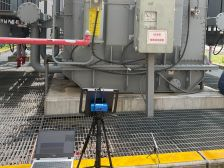
\includegraphics[width=1.0\linewidth]{equipment}
	\caption{Experimental platform for transformer acoustic signal acquisition at the substation.}
	\label{fig7}
\end{figure}

All experiments were run on a workstation with an Intel i9-14900K CPU and an NVIDIA RTX 5090 GPU (PyTorch 2.7, CUDA 12.8, Python 3.11).

\subsection{Evaluation Metrics}
All experiments report accuracy (Acc), weighted precision ($P_w$), weighted $F_1$-score ($F_1^w$), the geometric mean of per-class recalls
\begin{equation}
	G_{\text{mean}} = \left( \prod_{i=1}^{K} \frac{TP_i}{TP_i + FN_i} \right)^{\frac{1}{K}},
\end{equation}
and the inter-class standard deviations $\sigma_{P}$, $\sigma_{R}$, $\sigma_{F_1}$ (lower values indicate more uniform per-class performance). Results are mean $\pm$ std over five-fold stratified cross-validation.

\subsection{Experiment 1: GASF vs.\ GADF Feature Comparison}
\label{exp1}
Table~\ref{tab4} compares GASF and GADF inputs with and without PCNN (AlexNet-SE backbone). Without PCNN, Mel-GADF outperforms Mel-GASF (93.94\% vs.\ 92.42\% accuracy; $G_{\text{mean}}$ 0.9587 vs.\ 0.8503; $\sigma_{F_1}$ 0.0434 vs.\ 0.1490); with PCNN, both reach 96.97\%. GADF's difference-based encoding ($\sin(\phi_i - \phi_j)$) captures phase deviations more sensitively than the summation-based GASF ($\cos(\phi_i + \phi_j)$), and all subsequent experiments use the Mel-GADF-PCNN configuration.

\begin{table*}[ht]
	\centering
	\caption{Feature Comparison: GASF vs.\ GADF with and without PCNN (AlexNet-SE Backbone)}
	\label{tab4}
	\begin{tabular}{l l c c c c c c c}
		\toprule
		\multirow{2}{*}{Feature} & \multirow{2}{*}{PCNN} & \multicolumn{6}{c}{Evaluation Metrics} \\
		\cmidrule(lr){3-8}	
		&  & Acc(\%) & $P_w$(\%) & $F_1^w$ & $G_{\text{mean}}$ & $\sigma_{P}$ & $\sigma_{R}$ & $\sigma_{F_1}$ \\
		\midrule
		Mel-GADF & --   & 93.94 & 94.18 & 0.9392 & 0.9587 & 0.0591 & 0.0540 & 0.0434 \\
		Mel-GASF & --   & 92.42 & 93.73 & 0.9132 & 0.8503 & 0.0690 & 0.0222 & 0.1490 \\
		\midrule
		Mel-GADF & PCNN & 96.97 & 97.20 & 0.9684 & 0.9510 & 0.0308 & 0.0889 & 0.0485 \\
		Mel-GASF & PCNN & 96.97 & 97.22 & 0.9693 & 0.9736 & 0.0333 & 0.0500 & 0.0280 \\
		\bottomrule
	\end{tabular}
\end{table*}

\subsection{Experiment 2: Backbone Architecture Comparison with PINN}
\label{exp2}
Table~\ref{tab5} compares four backbones with the physics-informed framework on Mel-GADF-PCNN input. AlexNet-SE achieves the best performance (96.48\% accuracy, $F_1^w = 0.9649$, $G_{\text{mean}} = 0.9707$, $\sigma_{F_1} = 0.0133$); ResNet-18 and ConvNeXt-T follow at 95.45\%, while LeNet lags at 72.24\%. The confusion matrices in Fig.~\ref{fig11} show that AlexNet-SE misclassifies only one N0 sample.

\begin{table*}[ht]
	\centering
	\caption{Backbone Architecture Comparison with Physics-Informed Regularization (Mel-GADF-PCNN Input)}
	\label{tab5}
	\begin{tabular}{l c c c c c c c}
		\toprule
		\multirow{2}{*}{Backbone} & \multicolumn{6}{c}{Evaluation Metrics} \\
		\cmidrule(lr){2-7}	
		& Acc(\%) & $P_w$(\%) & $F_1^w$ & $G_{\text{mean}}$ & $\sigma_{P}$ & $\sigma_{R}$ & $\sigma_{F_1}$ \\
		\midrule
		PINN + LeNet      & 72.24 & 83.08 & 0.6718 & 0.5635 & 0.1944 & 0.3676 & 0.3226 \\
		PINN + ResNet-18  & 95.45 & 96.17 & 0.9548 & 0.9711 & 0.0632 & 0.0545 & 0.0391 \\
		PINN + ConvNeXt-T & 95.45 & 96.00 & 0.9536 & 0.9593 & 0.0480 & 0.0750 & 0.0428 \\
		PINN + AlexNet-SE & \textbf{96.48} & \textbf{96.57} & \textbf{0.9649} & \textbf{0.9707} & \textbf{0.0235} & \textbf{0.0182} & \textbf{0.0133} \\
		\bottomrule
	\end{tabular}
\end{table*}

\begin{figure*}[t]
	\centering
	\subfloat[]{\includegraphics[width=0.24\textwidth]{confusion_matrix1}}\hfill
	\subfloat[]{\includegraphics[width=0.24\textwidth]{confusion_matrix2}}\hfill
	\subfloat[]{\includegraphics[width=0.24\textwidth]{confusion_matrix3}}\hfill
	\subfloat[]{\includegraphics[width=0.24\textwidth]{confusion_matrix4}}
	\caption{Confusion matrices: (a) LeNet, (b) ResNet-18, (c) ConvNeXt-T, (d) AlexNet-SE. N0--Normal, N1--Short-circuit, N2--DC-bias, N3--Looseness, N4--Partial discharge.}
	\label{fig11}
\end{figure*}

\subsection{Experiment 3: Component-Wise Ablation Study}
\label{exp3}
Table~\ref{tab6} reports five incremental variants. SE attention contributes $+1.82\%$ accuracy over vanilla AlexNet, PCNN enhancement adds $+1.53\%$, and physics-informed regularization adds $+1.06\%$ with the largest $G_{\text{mean}}$ gain ($+0.0219$); the full model reduces $\sigma_{F_1}$ by 58\% versus the baseline (0.0133 vs.\ 0.0318).

\begin{table*}[ht]
	\centering
	\caption{Component-Wise Ablation Study (Mean $\pm$ Std over 5-Fold Cross-Validation)}
	\label{tab6}
	\footnotesize
	\begin{tabular*}{\textwidth}{@{\extracolsep\fill}l c c c c}
		\toprule
		\multirow{2}{*}{Model Variant} & \multicolumn{4}{c}{Metrics (mean $\pm$ std)} \\
		\cmidrule(lr){2-5}
		& Acc(\%) & $F_1^w$ & $G_{\text{mean}}$ & $\sigma_{F_1}$ \\
		\midrule
		(1) Baseline AlexNet           & $92.93 \pm 1.24$ & $0.9281 \pm 0.0131$ & $0.9264 \pm 0.0152$ & $0.0318 \pm 0.0082$ \\
		(2) + SE                       & $94.75 \pm 1.08$ & $0.9463 \pm 0.0114$ & $0.9491 \pm 0.0136$ & $0.0264 \pm 0.0068$ \\
		(3) + SE + PINN                & $95.73 \pm 0.95$ & $0.9561 \pm 0.0098$ & $0.9612 \pm 0.0112$ & $0.0215 \pm 0.0054$ \\
		(4) + SE + PCNN                & $96.20 \pm 0.88$ & $0.9608 \pm 0.0091$ & $0.9656 \pm 0.0104$ & $0.0192 \pm 0.0051$ \\
		(5) \textbf{Full (SE + PCNN + PINN)} & $\bm{97.26 \pm 0.82}$ & $\bm{0.9715 \pm 0.0084}$ & $\bm{0.9875 \pm 0.0098}$ & $\bm{0.0133 \pm 0.0042}$ \\
		\bottomrule
	\end{tabular*}
\end{table*}

\begin{table*}[ht]
	\centering
	\caption{Comparison with State-of-the-Art Methods (Mean $\pm$ Std over 5-Fold CV)}
	\label{tab7}
	\begin{tabular*}{\textwidth}{@{\extracolsep\fill}l c c c c}
		\toprule
		\multirow{2}{*}{Method} & \multicolumn{4}{c}{Metrics (mean $\pm$ std)} \\
		\cmidrule(lr){2-5}
		& Acc(\%) & $F_1^w$ & $G_{\text{mean}}$ & $\sigma_{F_1}$ \\
		\midrule
		SVM + PCA (Handcrafted)      & $82.57 \pm 2.14$ & $0.8214 \pm 0.0223$ & $0.7938 \pm 0.0256$ & -- \\
		1D-CNN (End-to-End, Raw)    & $87.14 \pm 1.86$ & $0.8692 \pm 0.0194$ & $0.8517 \pm 0.0213$ & $0.0681 \pm 0.0124$ \\
		EfficientNet-B0 (2D)        & $93.68 \pm 1.12$ & $0.9351 \pm 0.0118$ & $0.9423 \pm 0.0135$ & $0.0315 \pm 0.0072$ \\
		ViT-B/16 (2D)               & $94.11 \pm 1.08$ & $0.9398 \pm 0.0112$ & $0.9482 \pm 0.0128$ & $0.0298 \pm 0.0068$ \\
		ConvNeXt-T (2D)             & $94.92 \pm 1.02$ & $0.9476 \pm 0.0105$ & $0.9564 \pm 0.0116$ & $0.0256 \pm 0.0062$ \\
		Swin-T (2D)                 & $95.82 \pm 0.94$ & $0.9568 \pm 0.0098$ & $0.9689 \pm 0.0108$ & $0.0204 \pm 0.0054$ \\
		\textbf{Proposed (Ours)}    & $\bm{97.26 \pm 0.82}$ & $\bm{0.9715 \pm 0.0084}$ & $\bm{0.9875 \pm 0.0098}$ & $\bm{0.0133 \pm 0.0042}$ \\
		\bottomrule
	\end{tabular*}
\end{table*}

\subsection{Experiment 4: Comparison with State-of-the-Art Methods}
\label{exp4}
Benchmarked against seven representative methods under identical session-aware five-fold cross-validation (Table~\ref{tab7}), the end-to-end 1D-CNN ($87.14\%$) confirms the value of time--frequency representations; among modern architectures, Swin-T performs best ($95.82\%$), and the proposed method exceeds it by $+1.44\%$ ($p = 0.003$, paired $t$-test), showing that PCNN + PINN provide benefits beyond architectural innovation alone.

% \begin{figure*}
% 	\centering
% 	\includegraphics[width=1.0\linewidth]{drawing/fault-diagnosis/structure}
% 	\caption{Structure of the fault diagnosis module.}
% 	\label{fig10}
% \end{figure*}

% \subsection{Experiment 5: Hyperparameter Sensitivity Analysis}
% A systematic sensitivity analysis evaluated five key hyperparameters: gamma correction $\gamma$, PINN weight $\lambda_{\text{phy}}$, PCNN threshold $V_T$, PCNN iterations $N$, and learning rate. The macro $F_1$-score was evaluated across a grid of values using three-fold cross-validation. Key findings: $\gamma = 1.7$ provides optimal low-energy enhancement without over-saturation; $\lambda_{\text{phy}} = 0.1$ achieves the best data--physics balance (setting $\lambda_{\text{phy}} = 0$ yields $F_1 = 0.9608$, confirming the non-trivial benefit of the physical constraint); $V_T = 0.8$ balances noise suppression and feature preservation; $N = 10$ saturates performance with minimal computational overhead.

% \subsection{Experiment 6: Noise Robustness Evaluation}
% Models trained on clean data were evaluated under additive white Gaussian noise at SNR levels from $-5$~dB to $30$~dB. Four variants were compared: Baseline AlexNet-SE, +PINN (no PCNN), +PCNN (no PINN), and the Full model. At SNR $\geq 15$~dB, all variants maintain accuracy above $90\%$. At low SNR ($0$ to $5$~dB), PCNN-equipped variants outperform non-PCNN counterparts by $+5\%$ to $+8\%$. At SNR $= -5$~dB, the full model retains $78.3\%$ accuracy vs.\ $62.1\%$ for the baseline, a $+16.2\%$ improvement that highlights the synergistic benefit of combining biologically inspired denoising with physics-informed regularization.

\subsection{Discussion}
\textbf{Each component contributes non-trivially.} The ablation study (Table~\ref{tab6}) shows that SE attention, PCNN enhancement, and PINN regularization yield complementary gains, and their synergy achieves the best performance.

\textbf{Physics guidance and overfitting control.} The PINN term improves accuracy by $+1.06\%$ with the greatest effect on $G_{\text{mean}}$, validating the Laplacian smoothness prior; session-aware splits, dropout, weight decay, and the physics term keep the cross-validation spread at $\pm 0.82\%$. Limitations include the moderate dataset size (661 segments) and the first-order Laplacian prior; future work will pursue multi-site validation and the full Helmholtz equation with impedance boundary conditions.

\section{Conclusion}
\label{section6}
This paper presented a multi-modal acoustic fault diagnosis framework for power transformers integrating Mel-GADF three-channel fusion, PCNN-based denoising, and physics-informed Laplacian regularization within an improved AlexNet-SE backbone. On a real-world 220~kV transformer dataset, the full model achieves $97.26 \pm 0.82\%$ accuracy under session-aware five-fold cross-validation, outperforming Swin Transformer, ConvNeXt, and ViT by $+1.44\%$, $+2.34\%$, and $+3.15\%$, respectively. Future work includes multi-site validation with domain adaptation, higher-order acoustic physics, and lightweight edge-deployable variants.

\section{Acknowledgements}

This work is supported by the National Natural Science Foundation of China (No.~12404545), the Science Research Project of Hebei Education Department, China (No.~QN2025334), and the Fundamental Research Funds for the Central Universities (No.~2026MS144).

\section{Conflict of Interest}
On behalf of all authors, the corresponding author states that there is no conflict of interest.

\bibliography{references}

\end{document}

\endinput
